
%%%%%%%%%% Conference Latex Template for the university center of Tipaza - Algeria
%%%%%%%%%% created by F.CHABNI




\documentclass{paper}
\usepackage{ctex}
\usepackage{graphicx}
\usepackage{amsmath}
\usepackage{cite}
\usepackage{booktabs}
\title{自主移动车实现研究综述}
\author{邱璟祎, 周俊豪, 张峻瑜\\
  (按姓名首字母排序)
}
\begin{document}
\maketitle
\tableofcontents
\newpage
\section{引言}


\section{机械设计研究综述}
In this section, you describe the methods and procedures used in your research, including data collection, analysis, and interpretation\cite{YOUSFI2017789}.

\section{循迹研究综述}
\subsection{传统而有效的方法\cite{intro2023robot}}
\label{subsec:label}
\subsubsection{传感器:红外传感器、光敏电阻等}
\label{subsec:label}
红外传感器、光敏电阻等传感器实际上提供的传感能力是同质化的,此处以红外传感器为例介绍传统方法所用的传感器。

红外传感器是各种机器人比赛中最常见的传感设备。红外传感器可以发射红外光并接收反射光,根据反射光的强度输出电压。输出电压在经过有着固定基准值的电压比较器处理后将输出逻辑电平,便于控制器处理。
\begin{figure}[ht]
  \centering
  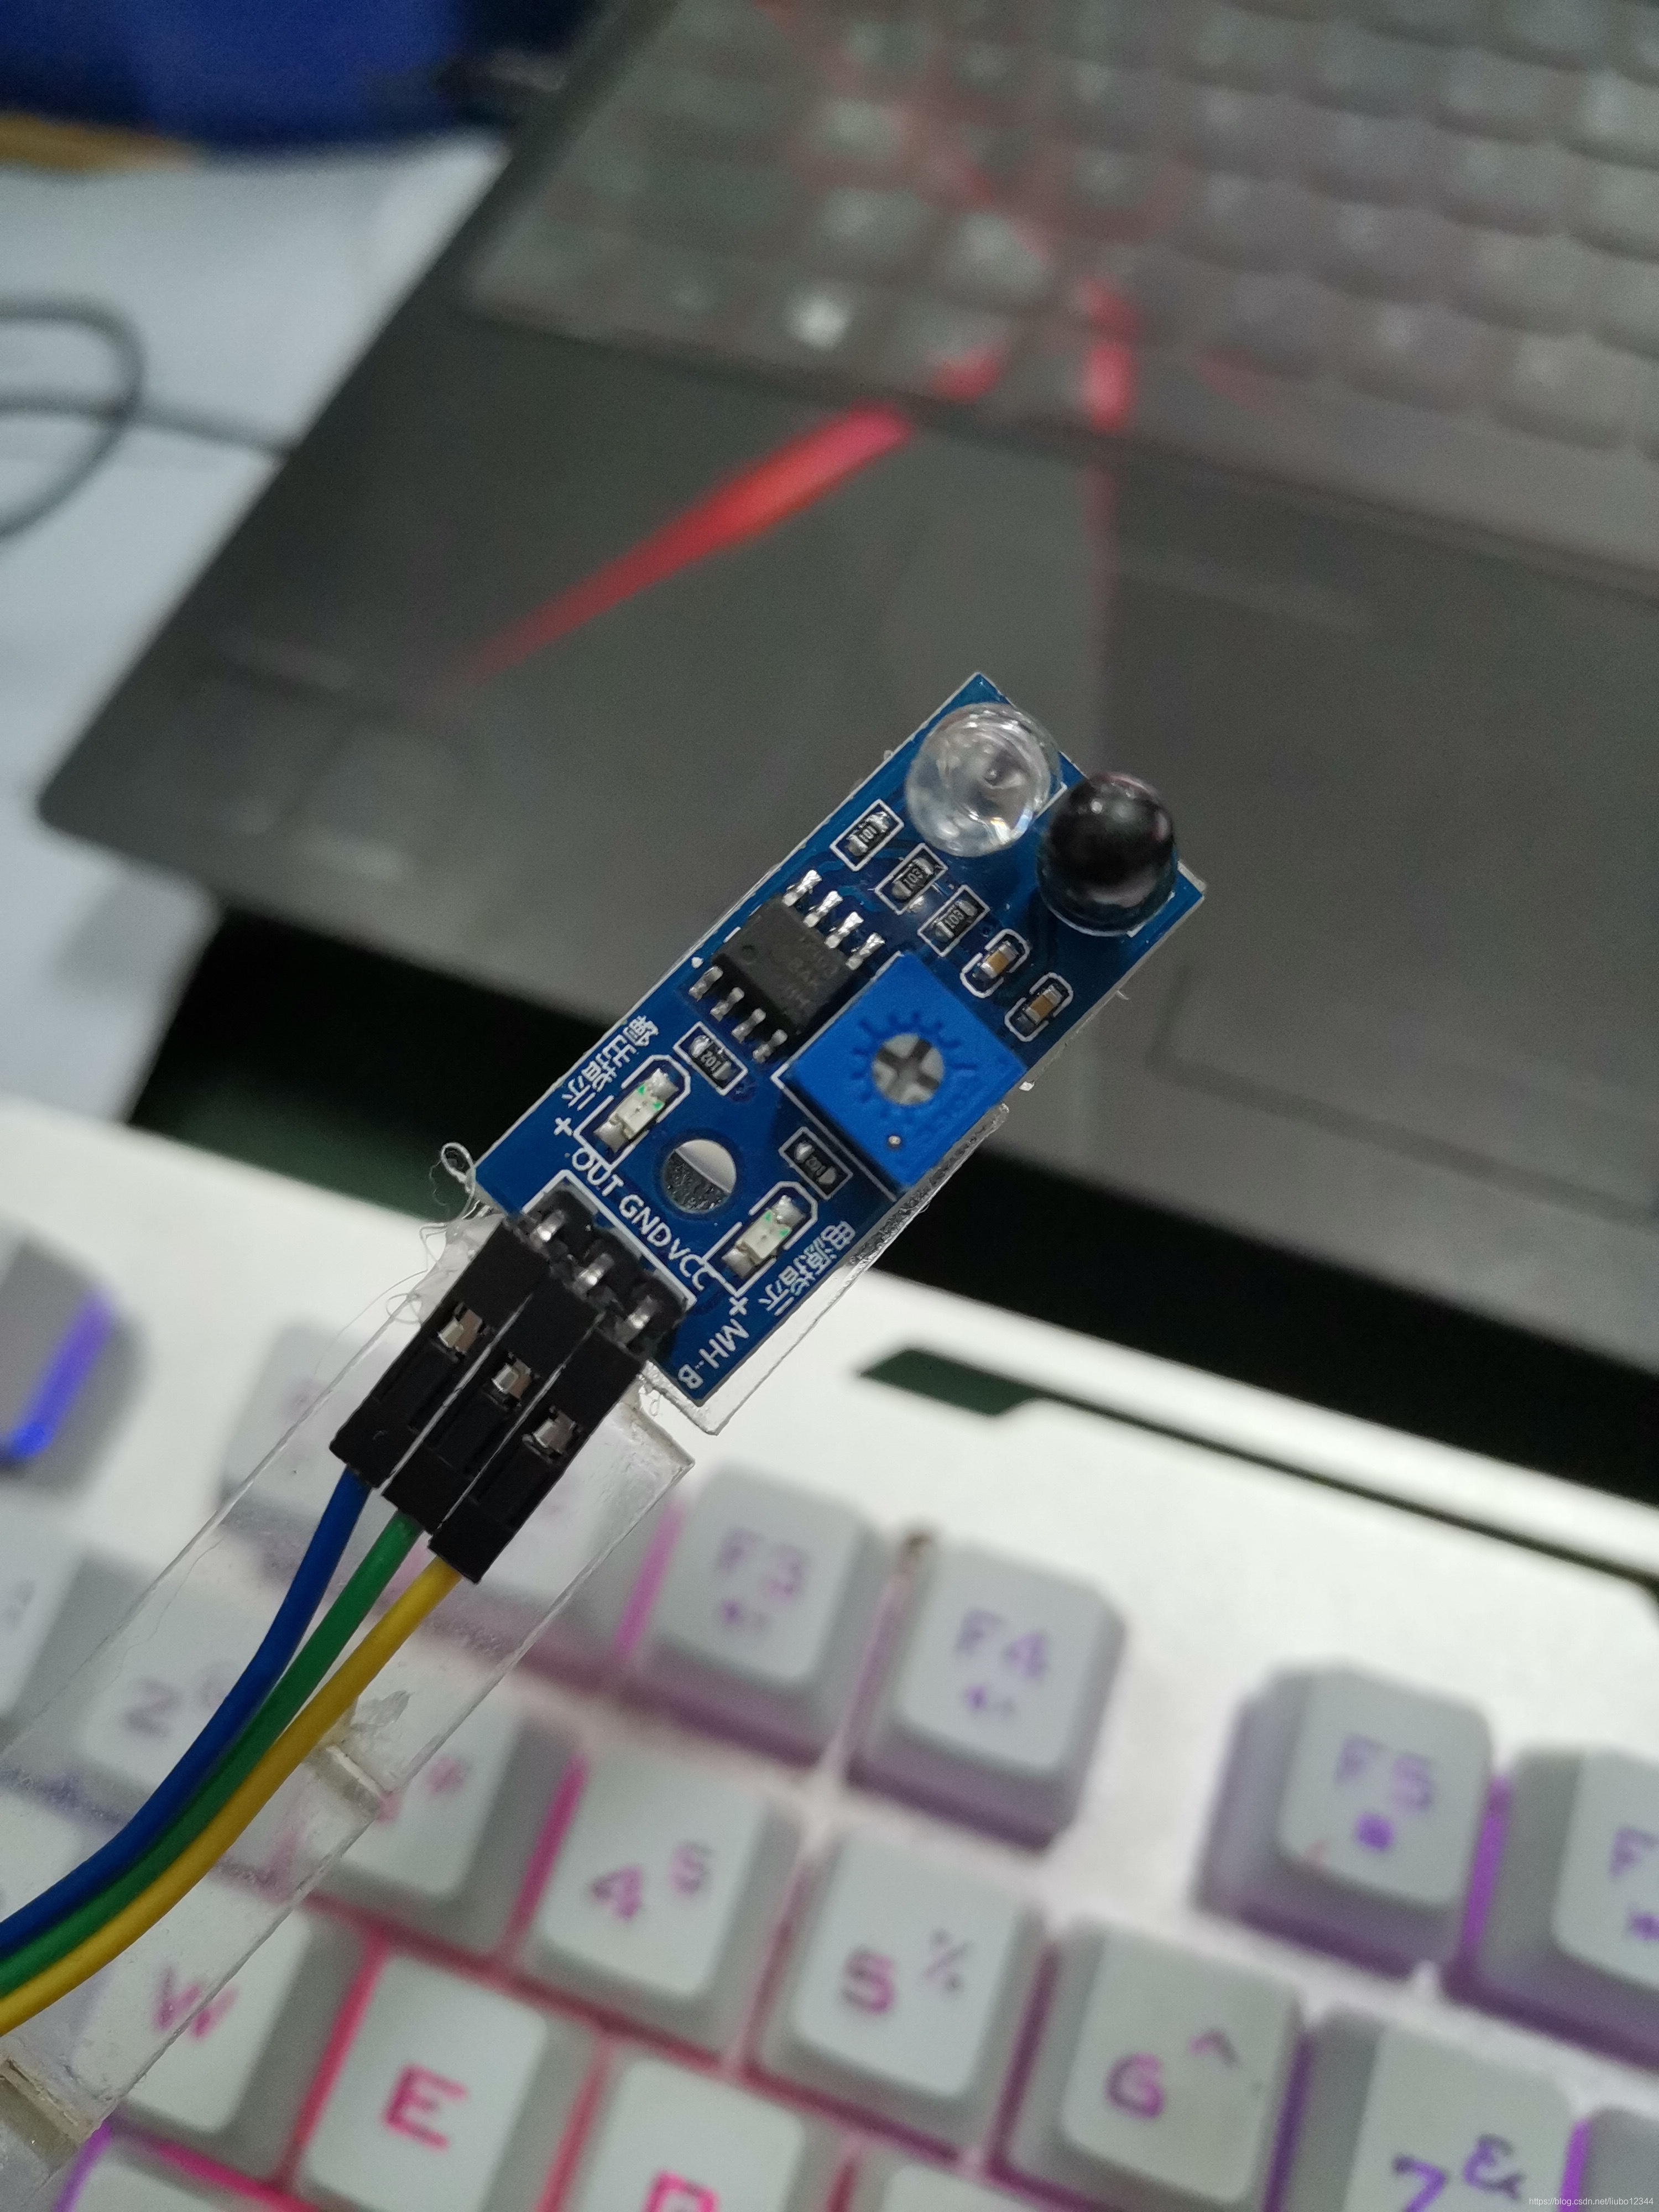
\includegraphics[width=0.5\textwidth]{figures/sensor.jpg}
  \caption{ 常见的红外传感器}
\end{figure}

常见的使用方案是在循迹车的前方布置对称的红外传感器。当线出现在红外传感器的正下方,它便会给控制电路采取行动的信号。例如当需要小车保持在黑色边线的赛道内时,如果侧边传感器有信号,则控制向另一个方向转弯。这种实现非常简单直观。

然而红外传感器的缺陷在于其只能给出是否检测到线的信息,而不能给出线的远近、角度信息,这使得它无法实现更加复杂和高效的控制算法。
\subsubsection{算法:从if-else到PID}
\label{subsec:label}
空间上离散的点观测传感器实际上提供了有限的状态数,只要根据状态给定行为就可以完成简单的控制。这只需要简单的if-else逻辑就能实现。但这样简单的方法代价是不够灵活,并且一个固定的控制指令并不能总是实现最优的控制。实际上的小车可能会困在反复地左右摇摆中浪费大量的时间和能量。

如果我们有一个点观测传感器组成的阵列或者进一步线性传感器,我们可以离散地或连续地得到与线之间的距离。这使得我们能够向循迹算法中引入PID。设定一个中间状态作为PID的基准,传感器阵列得到的距离可以作为PID的误差。利用PID控制两轮的转速差,使其小车保持在中间状态,可以实现更平滑、更快的循迹。

\subsection{更灵活高效的新方法}
\label{subsec:label}
2024年Yu Cao等人进行了深度强化学习循迹机器人的理论研究\cite{cao2024path}。他们将机器人与线路的横向偏差、机器人与路径之间的方向误差、机器人的速度和角速度等信息作为状态,而将机器人速度的变化率作为行动。在奖励函数中纳入与误差成正比的惩罚、与速度成正比的奖励以及惩罚机器人在困难弯道停下的参数。

\begin{figure}[ht]
  \centering
  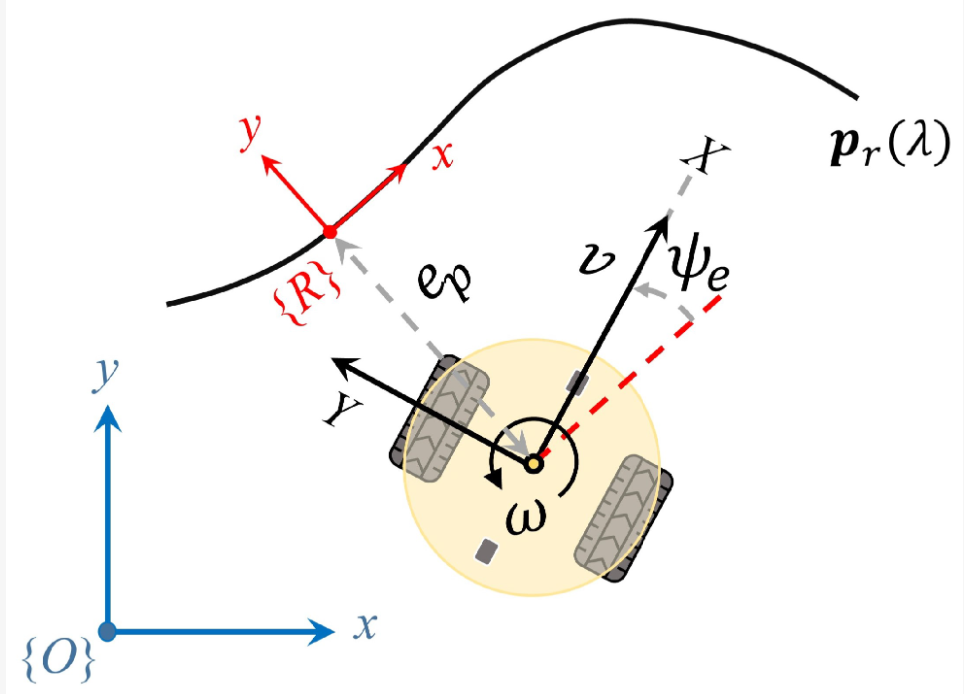
\includegraphics[width=0.5\textwidth]{figures/state.png}
  \caption{状态定义物理量\cite{cao2024path}}
\end{figure}

在随机生成的环境中进行了50万次交互之后,机器人的路径实现收敛。相比传统的PP控制方法,采用深度强化学习的机器人有了自适应的速度控制能力,可以适应不同曲率的路径,还有相当不错的泛化能力,在随机生成的不同路径中均有优秀的效果。

根据现实硬件情况在Webbot中建模并进行虚拟环境的预训练,再将完成训练的模型下载到实际小车中,就可以实现该方法的实际运用。
\section{避障研究综述}
\label{sec:label}



\section{讨论}
\section{结语}


\bibliographystyle{IEEEtran}
\bibliography{references}

\end{document}

%%% Local Variables:
%%% mode: LaTeX
%%% TeX-master: t
%%% End:
